\documentclass[10pt]{report}
\listfiles
\usepackage{amssymb}
\usepackage{amsmath}
\DeclareMathOperator*{\Max}{Max}
\usepackage{stmaryrd}
\usepackage{graphicx}
\usepackage{subfigure}
\usepackage{appendix}
\usepackage{algorithm}
\usepackage{algorithmic}
\usepackage{amsthm}
\usepackage[small]{caption}
\usepackage{cancel}
\usepackage{tikz} 
\usepackage{pgf}

%\usetikzlibrary{arrows,decorations.pathmorphing,backgrounds,positioning,fit,petri}

%%%% My Commands
\numberwithin{equation}{section}
%\usepackage[noprefix]{nomencl}
\newcommand{\eqnref}[1]{equation (\ref{#1})}                % Eq. (no)
\newcommand{\figref}[1]{Figure \ref{#1}}                % Figure (no)
\newcommand{\tblref}[1]{Table \ref{#1}}                % Table (no)
\newcommand{\secref}[1]{Section \ref{#1}}                % Section (no)
\newcommand{\incfig}{\centering\includegraphics*}  % Centered figure
\newcommand{\algref}[1]{Algorithm (\ref{#1})}
%DG integrals
\newcommand{\pd}[2]{\frac{ \partial #1}{\partial #2}}
\newcommand{\diff}[2]{\frac{d #1}{d #2}}
\newcommand{\fpd}[3]{\frac{ \partial #1}{\partial #2}_{\left [ #3\right] } }
\newcommand{\volint}[1]{ \sum_{k\in \mathcal{T}_{h}}\int_{\Omega_k} #1 d\Omega_{k} }  
\newcommand{\surfint}[1]{\sum_{i\in \mathcal{I}_{h}}\int_{\Gamma^{i}} #1 ds}
\newcommand{\esurfint}[1]{ \sum_{k\in \mathcal{T}_{h}}\oint_{\partial \Omega_{k} \backslash \Gamma^{b}} #1 ds}
\newcommand{\bsurfint}[1]{\sum_{b\in \mathcal{B}_{h}}\int_{\Gamma^{b}} #1 ds}
\newcommand{\bsurfintd}[1]{\sum_{b\in \mathcal{B}_{h}}\int_{\Gamma^{D}} #1 ds}
\newcommand{\bsurfintn}[1]{\sum_{b\in \mathcal{B}_{h}}\int_{\Gamma^{N}} #1 ds}
\newcommand{\frechd}[3]{ #1^{'}_{\left[ #2 \right]} \left( #3\right)} 
\newcommand{\adjd}[3]{ \pd{#1}{#2}_{\left[ #3 \right]}} 
\newcommand{\adjds}[2]{ #1_{#2}}
\newcommand{\frechds}[2]{ #1^{'}_{\left[#2 \right]} }
\newcommand{\innerp}[1]{\left< #1 \right>_{\Omega}}
\newcommand{\sinnerp}[1]{\left< #1 \right>_{\Gamma}}
% Operators
\newcommand{\diver}[1]{\nabla \cdot #1}
\newcommand{\laplace}[1]{\nabla^{2} #1}
\newcommand{\abs}[1]{\left| #1 \right|}
\newcommand{\avg}[1]{\left\{ #1 \right\} }
\newcommand{\jump}[1]{\llbracket #1 \rrbracket}
\newcommand{\mat}[1]{\left[ #1 \right]}
\newcommand{\paren}[1]{\left( #1 \right)}
\newcommand{\sparen}[1]{\left[ #1 \right]}
\newcommand{\sbracket}[1]{\left [ #1 \right] }
\newcommand{\twonorm}[1]{\parallel #1 \parallel_{2}}
\newcommand{\norm}[1]{\Vert  #1 \Vert}
\newcommand{\bignorm}[1] {\biggl \Vert  #1 \biggr \Vert}
\newcommand{\honenorm}[1]{\parallel #1 \parallel_{H^{1}}}
%variables
\newcommand{\hb}[1]{ {\bf #1}_{h} } % \hb for discrete symbol _{h} and bolded for vector in fields
% Fluxes 
\newcommand{\fc}{\vec{{\bf F}}_{c} \paren{\hb{u}}   }
\newcommand{\fv}{\vec{{\bf F}}_{v} \paren{\hb{u},\nabla \hb{u}} }
\newcommand{\fav}{\vec{{\bf F}}_{ad} \paren{ \epsilon,\hb{u},\nabla \hb{u} } }
\newcommand{\hc}{\mathcal{H}_{c} \paren{ \hb{u}^{+},\hb{u}^{-},\hb{v}^{+},\hb{v}^{-},\vec{n} } }  
\newcommand{\hv}{\mathcal{H}_{v} \paren{ \hb{u}^{+},\hb{u}^{-},\hb{v}^{+}, \hb{v}^{-},\nabla \hb{u}^{+},\nabla \hb{u}^{-},\vec{n} } }
\newcommand{\hav}{\mathcal{H}_{ad}\paren{ \epsilon^{+},\epsilon^{-},\hb{u}^{+},\hb{u}^{-}, \hb{v}^{+},\hb{v}^{-},\nabla \hb{u}^{+},\nabla \hb{u}^{-},\vec{n} } }
\newcommand{\hcb}{\mathcal{H}_{c}^{b} \paren{ \hb{u}^{b} \paren{ \hb{u}^{+} },\vec{n} } } 
\newcommand{\hvb}{\mathcal{H}_{v}^{b} \paren{ \hb{u}^{b} \paren{\hb{u}^{+}},\hb{v}^{+},\nabla \hb{u}^{+},\vec{n} } }
\newcommand{\havb}{\mathcal{H}_{ad}^{b} \paren{ \epsilon^{+}, \hb{u}^{b}\paren{ \hb{u}^{+}},{\bf v}_{h}^{+}, \nabla \hb{u}^{+},\vec{n} } }
% Proof environments
\newtheorem{prop}{Propositiion}

%Vocab
\newcommand{\node}{\texit{node}}
\newcommand{\elem}{\texit{element}}
\newcommand{\real}{\mathbb{R}}
% Constants
\newcommand{\half}[0]{\frac{1}{2}}                % Eq. (no)	
\newcommand{\gm}[0]{\paren{\gamma - 1}} 
\newcommand{\figwidth}{.47\textwidth} % small version .47, large version .6
\newcommand{\lfigwidth}{.68\textwidth} %small version .68, large verison .75
%%%%%%%%%%%%%%%%%%%%%%%%%%%%%%%%%%%
\begin{document}
 \title{Discontinuous Galerkin Methods}
 \date{\today}
 \author{Nick Burgess \\
  \emph{STC Corp. and U.S. Army Aeroflightdynamics Directorate}}
\maketitle

% Generate and print the lists
 \tableofcontents        % table of contents
 \listoffigures          % List of Figures
 \listoftables           % List of Tables
 % comment out line below if you have no program listings
 %\mylistoflistings      % List of program listings
 % Bring in the chapter files
\chapter{Introduction}
Discontinuous Galerkin (DG) methods are a particular type of finite-element method that is particularly well suited for convection dominated problems.  The name is derived from their close relationship to standard Galerkin finite-element methods.  However, in contrast to typical Galerkin finite-element methods no continuity requirements are imposed on the basis functions.  DG methods are a particularly attractive numerical method because they sit on a very solid mathematical background.  DG methods come equipped with all the standard finite-element method proofs of stability, consistency, and convergence at any discretization order.  This is a property that is not shared with finite-volume and similar unstructured grid numerical methods.  

DG methods are, in their most basic form, a finite-element method.  However, typical finite-element methods are continuous finite-element methods where the basis functions, which approximate the discrete solution, are continuous at the element interfaces.  Continuous finite-element methods traditionally have been applied to linear structural and thermal analysis problems that constitute purely elliptic operators, and hence continuous basis functions are appropriate.  DG methods employ basis functions that are discontinuous at the element interfaces, which makes DG methods naturally suitable for computing convection dominated problems.  DG discretizations are an ideal choice for convection dominated problems because the discontinuous basis functions allow for upwind flux calculations using approximate Riemann solvers.  Employing approximate Riemann solvers at the element interfaces is a strategy that is borrowed from finite-volume methods.  Thus DG can be thought of as a combination of traditional finite-element and finite-volume methods.  The blending of these methods is the result of simultaneously viewing the element as a control volume and as a domain over which interpolation functions (which are also known as basis functions) may be defined.  However, since the DG method is a finite-element method, the order of accuracy and number of unknowns are coupled.  DG methods attain high-order accuracy by adding additional basis functions within the elements, which results in additional degrees of freedom for increased orders of accuracy.  Alternatively, finite-volume and finite-difference methods reconstruct high-order data from neighboring elements, which does not increase the total number of degrees of freedom.  Therefore, finite-volume and finite-difference methods do not couple the order of accuracy with the number of degrees of freedom.  The coupling of the order of accuracy and number of unknowns within an element is a non-trivial property of DG methods, which affects many aspects of solver robustness and hence is a recurring theme throughout this work.   However, locating extra unknowns within the elements can be advantageous, provided that great care is taken in constructing and implementing these methods.     

As problem size increases, the efficient use of parallel computers becomes more important.  DG methods add resolution to a given problem via two approaches.  DG methods can add resolution by increasing the number of degrees of freedom within the element, which results in increased parallel efficiency over low-order methods for unstructured grids\cite{nastase07}.  By locating the DoFs within the element, higher computational density is achieved and proportionally less inter-element data communication is required.  This makes high-order DG methods an ideal candidate for large scale parallel computing.  Contrarily, while high-order finite-difference methods have been developed, these methods require the construction of extended interpolation stencils.  Extending the interpolation stencil can cause parallel scaling to degrade as the order of accuracy is increased.  This degradation of parallel efficiency is a result of the stencils of the grid points on partition boundaries relying on information from multiple data points on neighboring processors.  Reference \cite{nastase07} has shown that high-order DG methods have the opposite trend, as the order of accuracy increases the parallel scalability increases as well.       % chapter 1
\chapter{Finite-element Methods}
One of the principal reasons for choosing a discontinuous Galerkin(DG) method to approximate the solution of the partial differential equations is the solid mathematical background upon which these methods site.  In particular Galerkin's method can be shown to minimize a particular Sobolev norm of the error.  Furthermore, it can be shown that for a particular class of approximations, Galerkin's methods obtains the best approximation.  However, the price to be paid for this very solid mathematical theory is the mathematical formalism often used in explaining Galerkin's method, as well as the requirement of functional analysis for proving the stability, consistency and convergence of the numerical scheme.    

Discontinuous Galerkin (DG) methods are derived using a technique that is known as Galerkin's method.  Galerkin's method is a subset of a more general framework known as the method of weighted residuals (MWR).  While the MWR is usually introduced in the context of finite-element methods, it is in fact possible to show that finite-difference, finite-volume, spectral-collocation and a host of other methods can be derived using the MWR.  This allows one to study the relationship between these discretization methods and to draw conclusions about the suitability of certain methods for fluid dynamics problems.  

\section{Method of Weighted Residuals}
The method of weighted residuals is a general approach for solving differential equations.  The approach is to define a space in which one seeks an approximate solution (which is equivalent to  assuming a functional form of the solution).  We tend to denote this space $\mathcal{V}_{h}^{p}$.  In order to get a solid grasp of how the method of weighted residuals obtains an approximate solution consider the following one dimensional Poisson problem:
\begin{equation}\label{eq:c2_1dpoisson}
\frac{d^{2} u}{dx^{2}} + f(x) = 0, \quad x \in (a,b)
\end{equation}
subject to the Dirchlet boundary conditions
\begin{equation}
\begin{split}
& u(a) = g \\ 
& u(b) = h
\end{split}
\end{equation}
where it is assumed that f is a known scalar valued function on the interval  x = [a,b], which is the same as writing 
\begin{equation}
 f(x):[a,b] \rightarrow \mathbb{R} 
\end{equation}
which translated into english reads: ``f is a function such that(:) the input in a,b (inclusive) is mapped to some value in the space of real numbers''.  

While this notation can be tedious at first, once you work with finite-element methods enough it becomes quite natural to write things in this mathematical short hand.  Also this formality is not always necessary in an engineering context because engineers often assume that their function f(x) works in a certain space, such as the real numbers, as explained by the physics of the system in question.  However, for this very simple example we will be very formal so that the reader can appreciate that care must be taken when applying the MWR to solve differential equations.  

The method of weighted residuals seeks an approximate solution of this boundary value problem (which is a differential equation and boundary conditions) by considering an approximate solution $u_{h} \in \mathcal{V}_{h}^{p}$ to $u \in \mathcal{V}$ , where $\mathcal{V}_{h}^{p}$ is a chosen (and known) approximation space that should be contained inside of $\mathcal{V}$, \emph{i.e.} $\mathcal{V}_{h}^{p} \subset \mathcal{V}$ .  If one where to choose to employ monomials $1,x,x^{2},x^{3}...$ to generate $u_{h}$ then $\mathcal{V}_{h}^{p}$ is the space of monomials of degree $p$ defined on $h : x \in[a,b]$.  We will represent the discrete solution in a general form as a finite series summation 
\begin{equation}
u_{h}  = \sum_{i = 1}^{N} \hat{u}_{i} \phi_{i}(x)
\end{equation}
where the functions $\phi_{i}(x)$ are known as basis functions.  If one substitutes $u_{h}$ in place of $u$ in \eqnref{eq:c2_1dpoisson}, then since $u_{h}$ does not satisfy \eqnref{eq:c2_1dpoisson} there will be a residual or remainder defined by 
\begin{equation}
r(x) = \frac{d^{2} u_{h} }{dx^{2}} + f(x) \ne 0
\end{equation}     
The basic idea is to find the set of coefficients $\avg{ \hat{u}_{1}, \hat{u}_{2},...\hat{u}_{N} }$ that give you an approximate solution (hopefully this approximate solution is a good one?).  
The question is: how does one obtain these coefficients, because so far all we have is one residual statement and N unknown coefficients.  This is where the weighting comes into play.  The MWR defines the unknown coefficients $\avg{ \hat{u}_{1}, \hat{u}_{2},...\hat{u}_{N} }$ by requiring 
\begin{equation}
\int_{a}^{b} v_{i}(x) r(x)dx = 0 \quad \forall i = 1...N
\end{equation}
Essentially one picks a set of $N$ approximation functions $\avg{\phi_{i}(x)}$ and $N$ weighting functions $\avg{v_{i}(x)}$ and now one can solve a linear system to obtain the unknown coefficients $\avg{\hat{u}_{i}}$.  So far we have left the boundary conditions out of the problem.  One can either build these into the basis functions or into the coefficients.  While it is not immediately obvious from the mathematics so far, all numerical methods for ODEs/PDEs are the result of picking a certain choice of $v_{i}(x)$ and $\phi_{i}(x)$.  

\subsection{Galerkin's Method}
Now we are interested in Galerkin's method, which is defined by taking $v_{i}(x) = \phi_{i}(x)$:
\begin{equation}
\int_{a}^{b} \phi_{i}(x) r(x)dx = 0 \quad \forall i = 1...N
\end{equation}
The resulting discrete equations are given by 
\begin{equation}
\int_{a}^{b} \phi_{i} \paren{ \frac{d^{2} u_{h}}{dx^{2}} + f} dx = \int_{a}^{b}\phi_{i} \sum_{i=1}^{N} \hat{u}_{i} \frac{d^{2} \phi_{i} }{dx^{2}} + \phi_{i} f dx = 0 \quad \forall i = 1...N
\end{equation}
from which one can easily see that a system of linear algebraic equations for $\avg{u_{i}}$ is obtained.  This statement is sometimes referred to as Galerkin orthogonality because it is essentially defining the residual $r(x)$ such it is orthogonal to the space $\mathcal{V}_{h}^{p}$.    

While this seems like a particularly simple choice of $v_{i}(x)$ (which it is), it is not necessarily made because it's simple.  In fact this is the best choice of weight functions $v_{i}(x)$\footnote{The term test function is often used in the literature as a synonym for weight function either term is correct.}.  The best choice of weighting functions would be the functions which generate a discrete solution $u_{h}$ for all $x \in [a,b]$ which has the smallest norm $\norm{\cdot}$ of the error $e_{h} = u - u_{h}$.
Consider the equation governing the error(obtained by subtracting the discrete equation and the continuous one). 
\begin{equation}\label{eq:c2_poissonerr}
\frac{d^{2} u }{dx^{2}} + f - \frac{d^{2} u_{h}}{dx^{2}} - f = \frac{d^{2} \paren{u - u_{h}} }{dx^{2}} = \frac{d^{2} e_{h} }{dx^{2}} = 0 
\end{equation}
Taking the inner product over the domain [a,b] of the error equation \eqnref{eq:c2_poissonerr} with the error $e_{h}$ 
\begin{equation}
\int_{a}^{b} e_{h}\frac{ d^{2}e_{h}}{ dx^{2}}  dx = 0 
\end{equation}
integrating by parts and assuming no error at the boundaries ($\emph{i.e.}$ we assume that the approximate solution satisfies the boundary conditions exactly) gives 
\begin{equation}
\int_{a}^{b} \paren{ \frac{de_{h}}{dx}  }^{2} dx  = 0 
\end{equation}
which one should recognize as the $H^{1}$ Sobolev norm 
\begin{equation}
 \norm{u}_{H^{1}} = \paren{ \int \paren{ \frac{du}{dx}}^{2} dx }^{1/2}
\end{equation} 
 of the error e to the second power.  Recall that $e_{h}$ is a function of the coefficients $\avg{\hat{u}_{i}}$.  Therefore one can minimize the above Sobolev norm with respect to each of the coefficients $\avg{\hat{u}_{i}}$ 
 \begin{equation}
 \min_{\avg{\hat{u}_{i}}} \norm{e_{h}}_{H^{1}}^{2}
 \end{equation}
by differentiating the  $\norm{e_{h}}_{H^{1}}^{2}$ with respect to each of coefficients $\avg{\hat{u}_{i}}$
one obtains
\begin{equation}
\frac{ d\paren{ \norm{e_{h}}_{H^{1}}^{2} } } {d \hat{u}_{i}} = 2 \int_{a}^{b}-\paren{\frac{d e_{h} }{dx}  \frac{d \frac{d u_{h}}{dx} }{d \hat{u}_{i}} dx } = 0
\end{equation}
using 
\begin{equation}
\begin{split}
& \frac{d \frac{ d u_{h}}{dx} } {d \hat{u}_{i} } =\frac{d \phi_{i}}{dx}
\end{split}
\end{equation}
results in 
\begin{equation}
\begin{split}
& \frac{ d\paren{ \norm{e_{h}}_{H^{1}}^{2} } } {d \hat{u}_{i}} = - \int_{a}^{b} \frac{d \phi_{i}}{dx} \frac{d e_{h}}{dx} = \int_{a}^{b}  -\frac{d \phi_{i}}{dx} \paren{\frac{du}{dx} - \frac{d u_{h}}{dx}}  = 0
\end{split}
\end{equation}
which using integration by parts 
\begin{equation}
\begin{split}
& \int_{a}^{b} \frac{d \phi_{i}}{dx} \paren{-\frac{d u}{dx} + \frac{d u_{h}}{dx}} = \int_{a}^{b} -\frac{d \phi_{i}}{dx} \frac{d u_{h}}{dx} + \phi_{i} f dx =  \\
 & \int_{a}^{b} \phi_{i}\paren{ \frac{ d^{2} u_{h}}{dx^{2}} + f}dx  = 0 
 \end{split}
\end{equation}
which is what the MWR gave us to begin with.  Therefore, Galerkin's method gives the coefficients that minimize the error in the Sobolev norm $H^{1}$.  Furthermore in can be proven that this is the smallest possible error of all functions in $\mathcal{V}_{h}^{p}$.
\begin{prop}
The discrete solution $u_{h}$ is closer  to the exact solution $u$ than any other function in the space $\mathcal{V}_{h}^{p}$ under the $H_{1}$ Sobolev norm. 
\end{prop}
\begin{proof}
Staring with the discrete poisson equation given as 
\begin{equation*}
\int_{a}^{b} v_{h} \paren{ \frac{d^{2} u_{h} }{dx^{2}} + f(x) } = 0 \quad \forall v_{h} \in \mathcal{V}_{h}^{p}
\end{equation*}
since $\mathcal{V}_{h}^{p} \subset \mathcal{V}$ it is equally valid to define the weighted residual form of the poisson equation \eqnref{eq:c2_1dpoisson} as 
\begin{equation*}
\int_{a}^{b} v_{h} \paren{ \frac{d^{2} u}{dx^{2}} + f(x) }= 0 \quad \forall v_{h} \in \mathcal{V}_{h}^{p}
\end{equation*}
Subtracting these two equations 
\begin{equation*}
\int_{a}^{b} v_{h} \frac{d^{2} \paren{u - u_{h}} }{dx^{2}}= 0 \quad \forall v_{h} \in \mathcal{V}_{h}^{p}
\end{equation*}
which is the equation governing the error $e = u - u_{h}$.  Integration by parts results in the following weak form of the error equation
\begin{equation*}
\int_{a}^{b} \frac{d v_{h}}{dx} \frac{d \paren{u - u_{h}} }{dx}= 0 \quad \forall v_{h} \in \mathcal{V}_{h}^{p}
\end{equation*}
From here we take the Sobolev norm of the error $u - u_{h}$
\begin{equation*}
\bignorm{ \frac{ d \paren{u - u_{h}}}{dx}}^{2} = \int_{a}^{b} \paren{ \frac{ d \paren{u - u_{h}}}{dx}}^{2} dx
\end{equation*}
which can be re-written as 
\begin{equation*}
\int_{a}^{b} \paren{ \frac{ d\paren{u - u_{h}}}{dx}} \paren{\frac{  d\paren{u - v_{h}}}{dx}} -  \paren{\frac{ d\paren{u - u_{h}}}{dx}} \paren{\frac{  d\paren{u_{h} - v_{h}}}{dx}} dx
\end{equation*}
using the fact that 
\begin{equation*}
u_{h}, v_{h} \in \mathcal{V}_{h}^{p} \Rightarrow \paren{u_{h} - v_{h}} \in \mathcal{V}_{h}^{p}
\end{equation*}
gives
\begin{equation*}
\int_{a}^{b} \paren{\frac{ d\paren{u - u_{h}}}{dx}} \paren{\frac{  d\paren{u_{h} - v_{h}}}{dx}} dx = 0 
\end{equation*} 
by Galerkin orthongonality.  The remaining part of the norm is given as 
\begin{equation*}
\begin{split}
 & \bignorm{ \frac{ d \paren{u - u_{h}}}{dx} }^{2} = \int_{a}^{b} \paren{ \frac{ d\paren{u - u_{h}}}{dx}} \paren{\frac{  d\paren{u - v_{h}}}{dx}} dx \leq \bignorm{\frac{d \paren{u - u_{h}}} {dx}} \bignorm{\frac{d \paren{u - v_{h}}} {dx}} \\
 & \therefore \quad \bignorm{ \frac{ d \paren{u - u_{h}}}{dx}} \leq \bignorm{\frac{d \paren{u - v_{h}}} {dx}}  \quad \forall v_{h} \in \mathcal{V}_{h}^{p}
 \end{split}  
\end{equation*} 
\end{proof} 

One can see that for an arbitrary function $v_{h} \in \mathcal{V}_{h}^{p}$  we can prove that the error in the $H^{1}$ norm is larger than the $H^{1}$ norm of $u - u_{h}$.  This is really just a formal proof to show that while one can cast the Galerkin method as a minimization problem, one can also prove that this is the best solution in the approximation space.  Therefore, while choosing $v_{i} = \phi_{i}$ seems arbitrary and particularly simple at first, in fact this choice is the optimal one in some sense.  

The theory of MWR and finite-element methods is heavily based in functional analysis and finite-element methods are often used a motivation for mathematicians to examine certain types of functional analysis problems.  Vice versa utilizing finite-element and MWR methods require some basic understanding of functional analysis because it gives confidence in the results and provides reasons for why finite-element methods are defined in a particular fashion. 

\subsection{Briefly on Galerkin's Method and Continuity}
From the presentation in the previous section one should be tempted to ask: why integrate by parts?  This operation seems somewhat arbitrary and it is, to some extent.  However, consider that in order to approximate a second derivative the basis functions $\phi_{i}$ must be at least twice differentiable if integration by parts is not performed.
This is what is know as a continuity requirement.  In this case $\mathcal{C}^{1}$ continuity is required, which means that the function and it's first derivative must be continuous and differentiable.  However, if one integrates by parts once, then only first derivatives of the basis functions are required and the continuity requirement is reduced to $\mathcal{C}^{0}$, which states that the function itself must be continuous and differentiable (implying that the first derivative exists but is not necessarily differentiable).    It is convenient to try to minimize the highest derivative in the differential equation  by integrating by parts as many times as is advantageous.       

\subsection{Other MWR Based Methods}
So far we have seen the general form of the MWR method as well as the particular flavor known as Galerkin's method.  However, one can pick a variety of combinations for the basis and weighting functions.  For example if one selects the basis functions $\phi_{i}$ to be Lagrange polynomials $l_{i}$ defined at evenly spaced points in the domain $x \in [a,b]$ and  the weight functions to be the Dirac delta function $\delta\paren{x-x_{i}}$ defined at those same equally spaced points, then one obtained the finite-difference method.  Or if one picks the test function as the Heaviside function $H(x_{i})$ defined on sub intervals of the domain $x \in [x_{l},x_{h}] \subset [a,b]$ one obtains the so called sub-domain method (which can result in finite-volume and spectral volume-methods).  \tblref{tbl:c2_mwr} lists a few methods that are weighted residual methods based on the choice of weight function.   Obtaining other well known numerical methods often requires specifying the basis function as well as the weight function, e.g. collocation methods become finite-difference methods when the basis functions are Lagrange polynomials defined at the collocation points.   

\begin{table}[h!]
\caption{Various MWR methods for various choices of weight function}
\label{tbl:c2_mwr}
\center 
\begin{tabular}{|c|c|}
\hline  
Method & Weight Function \\
\hline 
Collocation & $\delta \paren{x - x_{i}} $ \\
Galerkin & Same as basis $\phi_{i}$ \\ 
Sub Domain & $H \paren{x - x_{i}}$ \\
Method of Moments & Monomials $1,x,x^{2}.....$ \\
\hline 
\end{tabular}
\end{table}

\subsection{A simple example of Galerkin's method for an ODE}
Consider the differential equation 
\begin{equation}
\frac{d^{2} u }{dx} + u = x^2
\end{equation}
on the domain $\Omega = x \in[0,1]$ subject to the non-homogenous boundary conditions 
\begin{equation} 
\begin{split} 
& u\paren{0} = 0 \\ 
& \frac{d u}{dx}\paren{1} = 1
\end{split}
\end{equation}
Up until now we have left the subject of boundary conditions relatively untouched and assumed that we can take these into account with the basis functions.  This problem will provide and example of how to accomplish this task.  For this second order differential equation we will consider a two term expansion of the form 
\begin{equation}
u_{h} = \hat{u}_{i} \paren{2x - x^{2}} + \hat{u}_{2}\paren{x^{2} + \frac{2}{3}x^{3}} 
\end{equation}
Examination of these functions shows that they satisfy the boundary condition at $x = 0$ since $\phi_{i}\paren{0} = 0, i = 1,2$.  However, these functions do not satisfy the boundary condition at $x = 1$ since $\frac{d \phi_{i}}{dx} \paren{1} = 0$.  Therefore in order we will introduce an extra function $\phi_{0} = 0$ to represent this boundary condition.  Sometimes in the literature adding boundary conditions in this fashion is known as adding a boundary lifting operator to the expansion.  Therefore the approximate solution is given by the modified or lifted expansion
\begin{equation}
u_{h} = x + \hat{u}_{1} \paren{2x - x^{2}} + \hat{u}_{2}\paren{x^{2} + \frac{2}{3}x^{3}} 
\end{equation}   
where the function $\phi_{0} = x$ does not have an unknown coefficient associated with it, rather the value is already known as 1.  Applying Galerkin's method 
\begin{equation}
\begin{split}
\int_{0}^{1} \phi_{i}\paren{ \frac{d^{2} u_{h} }{dx^{2}} + u - x^{2} } dx = 0 \quad i = 1,2
\end{split}
\end{equation}
Integration by parts
\begin{equation}
\int_{0}^{1} -\frac{d \phi_{i}}{dx} \frac{d u_{h} }{dx} + \phi_{i}u - \phi_{i} x^{2} dx = 0 \quad i = 1,2
\end{equation}
evaluating the integrals for i = 1 and i = 2 results in the following system of equations:
\begin{equation}
\begin{split}
& \frac{4}{5}\hat{u}_{1} + \frac{17}{20}\hat{u}_{2} = \frac{7}{60} \\
& \frac{17}{90}\hat{u}_{1} + \frac{29}{315} \hat{u}_{2} = \frac{1}{36} 
\end{split}
\end{equation}
Solving this system gives the unknown coefficients $\avg{\hat{u}_{i}}$:
\begin{equation}
\hat{u}_{1} = .154, \quad \hat{u}_{2} = 4.877e^{-3}
\end{equation}

\section{Classical Finite-element Methods}
Classical finite-element methods (FEM), which are sometimes referred to ask continuous Galerkin (CG) methods are simply a subset of the method of weighted residuals.  In this case the domain $\Omega$ is broken up into a set of canonical know shapes known as elements such that
\begin{equation}
\Omega = \cup_{e} \Omega_{e}
\end{equation}
where $\Omega_{e}$ is a single element.  In one dimension those elements are called bars or bar elements.  In two dimensions the elements are usually triangles or quadrilaterals.  However, other shapes are possible provided one can define basis functions that satisfy the requirements of the FEM and physical problem.  In three dimensions many element shapes are possible including: tetrahedra, hexahedra, pyramids and prisms.  

For a CG method the basis functions, which have compact support (a fancy way of saying the basis functions are non-zero on only one element of the domain) are defined the elements and the residual is weighted with all basis functions in the domain.  Classically finite-elements using linear Lagrange polynomials which are value one at the one node in the element.  Therefore, each element has two non-zero basis functions.  The basis functions are illustrated in \figref{fig:c2_1d_lagrange}. 
\begin{figure}[h!]
\centering
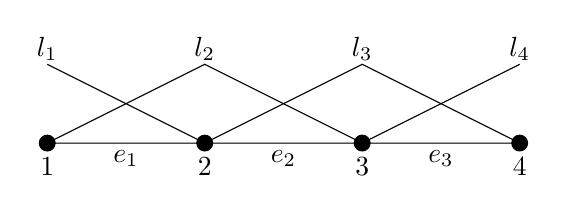
\begin{tikzpicture}
%\draw (-1.5,0) -- (1.5,0);
%\draw (0,-1.5) -- (0,1.5);
%  Draw nodes and lines that connect them
\draw[fill=black] (0,0) circle (.1cm)  -- (2,0) circle (.1cm)  -- (4,0) circle (.1cm)  -- (6,0) circle (.1cm);
\draw (0, -.3) node {1};
\draw (2, -.3) node {2};
\draw (4, -.3) node {3};
\draw (6, -.3) node {4};
%  Now label the 3 elements
\draw (1,-.2) node {$e_{1}$} (3,-.2) node {$e_{2}$} (5,-.2) node {$e_{3}$};
% l_{1}
\draw (0,1) -- (2,0);
\draw (0,1.2) node {$l_{1}$};
% l_{2}
\draw (0,0)
-- (2,1) 
-- (4,0);
\draw (2,1.2) node {$l_{2}$};
% l_{3}
\draw (2,0) -- (4,1) -- (6,0);
\draw (4,1.2) node {$l_{3}$};
% l_{4}
\draw (4,0) -- (6,1);
\draw (6,1.2) node {$l_{4}$};
\end{tikzpicture}
\caption{Example of linear Lagrange or so-called hat functions defined locally on the elements in a mesh}
\label{fig:c2_1d_lagrange}
\end{figure}



\begin{figure}[h!]
\centering
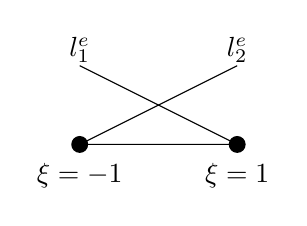
\begin{tikzpicture}
\draw[fill = black]  (0,0) circle (.1cm) -- (2,0) circle(.1cm) ;
\draw (0,-.4) node {$\xi = -1$} (2,-.4) node {$\xi = 1$};
% l_{1}
\draw (0,1) -- (2,0); \draw (0,1.2) node {$l^{e}_{1}$};
% l_{2}
\draw (0,0) -- (2,1) ; \draw (2,1.2) node {$l^{e}_{2}$};
\end{tikzpicture}
\caption{Standard element and local basis functions}
\label{fig:c2_standard_elem}
\end{figure}

For an element the basis functions are given by the formulas
\begin{equation}
\begin{split}
& l^{e}_{1} = \frac{1 - \xi}{2} \quad \xi \in [-1,1] \\
& l^{e}_{2} = \frac{1+ \xi}{2} \quad \xi \in [-1.1]
\end{split}
\end{equation}
where these formulas are given in the so called standard element using the standard or parametric coordinate $\xi$.  The standard element depicted in \figref{fig:c2_standard_elem} is mapped to the physical one using the relation
\begin{equation}
x = l^{e}_{1}x_{1} + l^{e}_{2}x_{2}
\end{equation}
 where $x_{1}$ is coordinate at the left end of the element and $x_{2}$ is the coordinate at the right end of the element. 
 
 Let's consider the Poisson equation in \eqnref{eq:c2_1dpoisson} and discretize it using a general finite-element method.  Formally we state the finite-element problem as find $u_{h} \in \mathcal{V}_{h}$ such that
\begin{equation}\label{eq:c2_pois_fem}
\int_{\Omega} v_{h} \paren{ \frac{d^{2} u_{h}} {dx^{2}} - f(x) } = 0 \quad \forall v_{h} \in \mathcal{V}_{h}
\end{equation}

While the residual is weighted with each test function and integrated over the domain globally in practice only integrals over the elements need to be computed since most of the basis functions are zero on a particular element.  Recalling that the domain $\Omega$ is the union of elements $\Omega_{e}$ \eqnref{eq:c2_pois_fem} can be writtten as 
\begin{equation}
\sum_{e} \int_{\Omega_{e}} v_{h} \paren{ \frac{d^{2} u_{h}}{dx^{2}} - f\paren{x}} d\Omega_{e} = 0 \quad \forall v_{h} \in \mathcal{V}_{h}
\end{equation}
Applying integration by parts yields:
\begin{equation}\label{eq:c2_pois_fem_weak}
\sum_{k}\int_{\Omega_{e} } -\diff{v_{h}}{x}\diff{u_{h}}{x} - v_{h} f(x) d \Omega_{e} + v_{h}\diff{u_{h}}{x} {\vert_{\xi = -1}^{\xi=1}}_{k}= 0 \quad \forall v_{h} \in \mathcal{V}_{h}
\end{equation}
 where the term evaluated at $\xi = -1,1$ is evaluated at the element boundaries.  The term evaluated at the element boundaries normally cancels out due to the continuity of the basis functions.  To see how this is accomplished consider a collection of elements donated $k = 1, 2, 3$ in \figref{fig:c2_1d_lagrange}.  One now selects the $v_{h}$ as $l_{2}$.  The summation over elements in \eqnref{eq:c2_pois_fem_weak} becomes 
 \begin{equation}
 \begin{split}
 & \sum_{k}\int_{\Omega_{e} } -\diff{l_{2}}{x}\diff{u_{h}}{x} - l_{2} f(x) d \Omega_{e} + l_{2}\diff{u_{h}}{x} \vert_{x_{1}}^{x_{2}}= \\
 & \int_{\Omega_{1} } -\diff{l_{2}}{x}\diff{u_{h}}{x} - l_{2} f(x) d \Omega_{e} + l_{2}\diff{u_{h}}{x}  \vert_{x_{1}}^{x_{2}} + \\ 
 & \int_{\Omega_{2} } -\diff{l_{2}}{x}\diff{u_{h}}{x} - l_{2} f(x) d \Omega_{e} + l_{2}\diff{u_{h}}{x}  \vert_{x_{2}}^{x_{3}}
 \end{split}
 \end{equation}
 Since we are using a Galerkin method the form of $u_{h}$ is given as 
 \begin{equation}
 u_{h} = \sum_{j} \hat{u}_{j} l_{j}\paren{x}
 \end{equation}
 where $j = 1,2$ locally on each element.  Using the known form of $u_{h}$ results in 
 \begin{equation}
 \begin{split}
 &\int_{\Omega_{1} } -\diff{l_{2}}{x}\diff{u_{h}}{x} - l_{2} f(x) d \Omega_{1} + 1\paren{ \hat{u}_{1} \diff{l_{1}}{x} + \bcancel{\hat{u}_{2}\diff{l_{2}}{x}} }  -\cancel{ 0\paren{  \hat{u}_{1} \diff{l_{1}}{x} + \hat{u}_{2}\diff{l_{2}}{x} } }+ \\ 
  &\int_{\Omega_{2} } -\diff{l_{2}}{x}\diff{u_{h}}{x} - l_{2} f(x) d \Omega_{2} + \cancel{0\paren{ \hat{u}_{2} \diff{l_{2}}{x} + \hat{u}_{3}\diff{l_{3}}{x} } } - 1\paren{ \bcancel{ \hat{u}_{2} \diff{l_{2}}{x}} + \hat{u}_{3}\diff{l_{3}}{x} }
 \end{split}
 \end{equation}
 where we have simply employed the property of the basis functions:
 \begin{equation}
 l_{j}\paren{x_{i}} = \delta_{ij}
\end{equation}
This type of patter is repeated from element to element through the domain.  As the integrals are performed the boundary terms cancel out.  This canceling out is due to the continuity of the basis functions $l_{j}$.  The method of forming the residual at a node (node 2 in this case) is used as a demonstration of how the inter-element boundary terms cancel out formally.

\subsection{Implementation}
In practice one does not normally go through the formal crossing out of the inter element boundary contributions to the discrete residual.  In practice these surface terms are ignored and one forms integrals over the elements and then added the contributions the nodes that make up the element.  This gives rise to the so-called element matrices that are so common in textbooks on FEM.  Continuing with the poisson equation example the two element residual equations for element $k = 2$ are
\begin{equation}
\begin{split}
& \int_{\Omega_{2} } -\diff{l_{2}}{x} \diff{u_{h}}{x} - l_{2} f(x) d \Omega_{2} \\
& \int_{\Omega_{2} } -\diff{l_{3}}{x} \diff{u_{h}}{x} - l_{3} f(x) d \Omega_{2} 
\end{split}
\end{equation}
if one recalls that 
\begin{equation}
 u_{h} = \sum_{j} \hat{u}_{j} l_{j}\paren{x}
\end{equation}
then the equations for an element are written in matrix form as 
\begin{equation}\label{eq:c2_elem_mat}
\left[
\begin{array}{cc}
-\int_{\Omega_{2}} \diff{l_{2}}{x} \diff{l_{2}}{x} dx & -\int_{\Omega_{2}} \diff{l_{2}}{x} \diff{l_{3}}{x} dx \\
-\int_{\Omega_{2}} \diff{l_{3}}{x} \diff{l_{2}}{x} dx & -\int_{\Omega_{2}} \diff{l_{3}}{x} \diff{l_{3}}{x} dx
\end{array}
\right]
\left\{
\begin{array}{c}
\hat{u}_{2} \\ 
\hat{u}_{3} 
\end{array}
\right\} = 
\left\{
\begin{array}{c}
\int_{\Omega_{2}} l_{2} f(x) dx \\
\int_{\Omega_{2}} l_{3} f(x) dx 
\end{array}
\right\}
\end{equation}

The matrix in \eqnref{eq:c2_elem_mat} is know as the element stiffness matrix.  One should immediately note that element 2 in this case involves the unknowns as nodes 2 and 3.  However these nodes also have contributions from other elements.  Recall that in reality we should have written the equations on a per node basis since these are the unknowns for this particular finite-element approach.  However, we can properly recover the equations for each node by properly combining the element element matrix equations using a process known as global matrix assembly.  One should also be aware that both the element and global matrices are often referred to as stiffness matrices in the literature.  This nomenclature is taken from the structural analysis fields where continuous Galerkin methods were first applied.  


\subsubsection{Global Matrix assembly}
In one spatial dimension it is easy to demonstrate how the global matrix assembled from the local element matrices.  The matrix equations in \eqnref{eq:c2_elem_mat} are in fact just the local equations for element 2.  These equations can be written symbolically as 
\begin{equation}
\left[k^{e}\right]  \left\{ \hat{u}^{e} \right\} = \left\{ f^{e} \right\}
\end{equation} 
for each element $e$ in the mesh.  Examination of the finite-element mesh in \figref{fig:c2_1d_lagrange} gives an indication of how the global matrix assembly works.  In this case each node is connected to two elements.  Therefore each node's diagonal matrix entry will be the sum of contributions from both element's connected to it.  There will be no off-diagonal addition entries because the elements are only connected by nodes.  If this were a 2-D triangular mesh the entries of the matrix that are additions from various elements would be more complicated since elements are connected by edges in this higher dimensional space.  The assembly of the global system for the example mesh in \figref{fig:c2_1d_lagrange} is illustrated as 
\begin{equation}
\left[ 
\begin{array}{cccc}
k^{1}_{11} & k^{1}_{12} & 0 & 0 \\
k^{1}_{21} & k^{1}_{22} + k^{2}_{11}  & k^{2}_{12} & 0 \\
0 & k^{2}_{21} & k^{2}_{22} + k^{3}_{11}  & k^{3}_{12} \\
0 & 0 & k^{3}_{21}  & k^{3}_{22} \\
\end{array}
\right] 
\left\{
\begin{array}{c}
\hat{u}_{1} \\ 
\hat{u}_{2} \\
\hat{u}_{3} \\
\hat{u}_{4} \\
\end{array} 
\right\} = 
\left\{
\begin{array}{c}
f^{1}_{1} \\
f^{1}_{2} + f^{2}_{1} \\ 
f^{2}_{2} + f^{3}_{1} \\
f^{3}_{1}
\end{array}
\right\}
\end{equation}
Essentially this indexing of the global matrix takes advantage of what is know as the mapping from the local node number to the global node number.  If one considers an element say element 2 in the global mesh
\begin{figure}[h!]
\centering
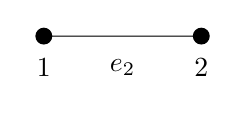
\begin{tikzpicture}
\draw[fill = black] (0,0) circle (.1cm) -- (2,0) circle (.1cm) ;
\draw (1,-.4) node {$e_{2}$};
\draw (0,-.4) node {1} (2,-.4) node {2};
\end{tikzpicture}
\caption{Local and global node numbering }
\label{fig:c2_local_global_num}
\end{figure}
and we observe that local node 1 in this case is global node 2 and local node 2 is global node 3.  

Each element in the mesh has 2 nodes denoted 1 and 2 and these nodes have a corresponding global node number.  The element stiffness matrix entries indexed as $k^{e}_{ij}$ reflect the local number numbering on each element and then are added to the rows and columns of the global matrix by considering the global node numbers of the nodes belonging to each element.  The $i,j$ in the local element stiffness matrices can be considered as the effect of local node $j$ on the solution at node $i$.  So in the case of element 2 we take the element stiffness matrix $\left[k^{e}\right]$ and add it the global system $\left[k \right]$ as: 
\begin{equation}
 \begin{split} 
 k_{22} += k^{2}_{11} \\
 k_{23} += k^{2}_{12} \\
 k_{32} += k^{2}_{21} \\
 k_{33} += k^{2}_{22} \\
 \end{split}
 \end{equation}
 
For more complicated meshes there exists a formal assembly algorithm for 2/3-D meshes employing linear elements.  One could in theory develop such an algorithm for any type of continuous finite-element discretization.  

\chapter{Mesh Data Structures}
This chapter describes the mesh data structures that are implemented as part of the class UnstGrid.  \textbf{UnstGrid} is a C++ class defined in the file \underline{UnstGrid.h}.  If you're interested in the source documentation please see the source code manual. 

\section{Introduction} 
For the purposes of this document a mesh denotes a collection of nodes and elements.  nodes define points in physical space and elements describe how these nodes are connected.  The FEM library only supports certain types elements i.e. 1-D lines, 2-D triangles, 2-D quadrilaterals, 3-D tetrahedra, 3-D prisms, and 3-D Hexahedra.  First we describe how elements are defined and how they are combined to form unstructured meshes.  Then with the theory how meshes are defined in hand we will describe the data structures used in the code to define them and how to acess the data of the mesh using the implemented class functions of \textbf{UnstGrid}. 

Note that mesh generation is a topic unto itself and the goal of this section is to describe how the numerical integration library interacts with a pre-existing mesh.  A pre-existing mesh is one where the nodal coordinates in the physical space (i.e. the one in which we wish to solve the PDE's) represented notionally by the coordinates $(x,y,z)$ are known.  Additionally a mesh must supply how these nodes are connected into elements along with how the boundary faces of the domain are connected to the nodes that lie on the domain boundary.  A few conditions on the mesh are that is must be completely fill the domain of interest $\Omega$, mathematicaly this is 
\begin{equation}
\Omega = \bigcup_{e} \Omega_{e}
\end{equation}  

\section{Element Types}
This section describes the types of elements that are supported by the solver library.  In general elements define how nodes in the mesh are connected to each other.  Elements are normally defineds in a know standard space defined by greek letters $\xi, \eta, \zeta$.  The positions of the nodes of the elements are known in this standard space and the physical locations of the nodes in $(x,y,z)$ spaces are determined by a mapping function $f_{m}: \real^{d}\rightarrow \real^{d} $ where $d$ is the number of physical dimensions of the domain.  In this work the mapping functions $f_{m}$ take on the form of polynomial interpolations, that are nodally exact at all nodes of the element.       
 
\subsection{1-D Bar}
In one spatial dimension only one type of element is available.  This element in known as the ``bar'' element.  The ``bar'' element (shown in \figref{fig:c3_line}) is constructured by taking two nodes of the mesh and connecting them by a line segment.  
\begin{figure}[h!]
\centering
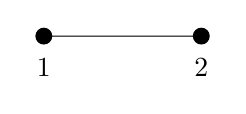
\begin{tikzpicture}
\draw[fill = black]  (0,0) circle (.1cm) -- (2,0) circle(.1cm) ;
\draw (0,-.4) node {1} (2,-.4) node {2};
\end{tikzpicture}
\caption{1-D ``bar'' element.}
\label{fig:c3_line}
\end{figure}

Recalling that each element has a definition in the standard space of equivalent dimension the coordinates of the nodes are node$_{1}$: $\xi = -1$ and node$_{2}$: $\xi = 1$ in the standard space spanning $\xi \in (-1,1)$.  

A 1-D ``bar'' element may have any number of solution unknowns associated with it but it requires a minimum of two uknowns: one for each element of the element.  For finite-element methods this results in a linear data representation and an asymptotically second-order accurate solution.  

\subsection{2-D Triangle}
In two spatial dimensions there are two element types available one of which is the triangle.  The triangle is defined by connecting 3 of the mesh nodes as in \figref{fig:triangle}.  

 



\section{Mesh Connectivity}
The mesh connectivity data is stored in a linked list structure to facilitate optimal memory footprint.  Each connectivity of the mesh is stored as a separate linked list.  For example the nodes belonging to an element is one mesh connectivity and is stored in one linked list while the elements surrounding a node is stored in yet another linked list.  Each linked list is comprised of two arrays an ``index'' array and a ``data'' array.  The index array is normally named with an ``i'' at the end of the variable name and is composed on integer. 

As an example consider the connectivity defining the node numbers of each element in a mesh.  To make the explanation concrete consider the simple mesh in \figref{fig:c3_sample_mesh}.  
\begin{figure}[h!]
\centering
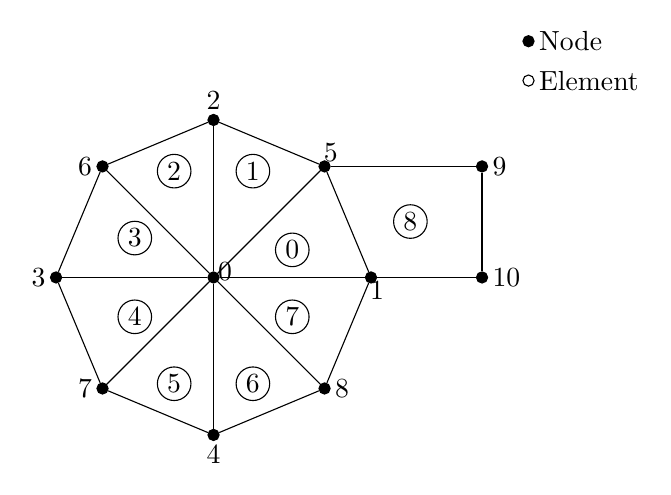
\begin{tikzpicture}[inner sep=.5mm,minimum size=.5mm]
\node at (0,0) [circle,draw=black,fill=black] (Node1) {};
\node at (2,0) [circle,draw=black,fill=black] (Node2) {};
\node at (0,2) [circle,draw=black,fill=black] (Node3) {};
\node at (-2,0) [circle,draw=black,fill=black] (Node4) {};
\node at (0,-2) [circle,draw=black,fill=black] (Node5) {};
\node at ( 1.41,1.41) [circle,draw=black,fill=black] (Node6) {};
\node at (-1.41,1.41) [circle,draw=black,fill=black] (Node7) {};
\node at (-1.41,-1.41) [circle,draw=black,fill=black] (Node8) {};
\node at (1.41,-1.41) [circle,draw=black,fill=black] (Node9) {};
\node at (3.41,1.41) [circle,draw=black,fill=black] (Node10) {};
\node at (3.41,0) [circle,draw=black,fill=black] (Node11) {};
\node [black,right] at (Node1.north) {0};
\node [black,below] at (Node2.east) {1};
\node [black,above] at (Node3.north) {2};
\node [black,left] at (Node4.west) {3};
\node [black,below] at (Node5.south) {4};
\node [black,above] at (Node6.east) {5};
\node [black,left] at (Node7.west) {6};
\node [black,left] at (Node8.west) {7};
\node [black,right] at (Node9.east) {8};
\node [black,right] at (Node10.east) {9};
\node [black,right] at (Node11.east) {10};
\draw (Node1) -- (Node2);
\draw (Node1) -- (Node3);
\draw (Node1) -- (Node4);
\draw (Node1) -- (Node5);
\draw (Node1) -- (Node6);
\draw (Node1) -- (Node7);
\draw (Node1) -- (Node8);
\draw (Node1) -- (Node9);
\draw (Node2) -- (Node6);
\draw (Node6) -- (Node3);
\draw (Node3) -- (Node7);
\draw (Node7) -- (Node4);
\draw (Node4) -- (Node8);
\draw (Node8) -- (Node5);
\draw (Node5) -- (Node9);
\draw (Node9) -- (Node2);
\draw (Node6) -- (Node10);
\draw (Node10) -- (Node11);
\draw (Node11) -- (Node2);
\node at (1,.35) [circle,draw=black] (elem1){0};
\node at (.5,1.35) [circle,draw=black] (elem2){1};
\node at (-.5,1.35) [circle,draw=black] (elem3){2};
\node at (-1,.5) [circle,draw=black] (elem4){3};
\node at (-1,-.5) [circle,draw=black] (elem5){4};
\node at (-.5,-1.35) [circle,draw=black] (elem6){5};
\node at (.5,-1.35) [circle,draw=black] (elem7){6};
\node at (1,-.5) [circle,draw=black] (elem8){7};
\node at (2.5,.71) [circle,draw=black] (elem9){8};
\node at (4,3) [circle,draw=black,fill=black] (nodelegend) {};
\node at (4,2.5) [circle,draw=black] (elemlegend) {};
\node  [black,right] at (nodelegend.east) {Node};
\node  [black,right] at (elemlegend.east) {Element} ;
\end{tikzpicture}
\caption{Sample Mesh.}
\label{fig:c3_sample_mesh}
\end{figure}
One should note that this 2-D example contains a mesh of mostly triangles with one quadrilateral.  The mixed element nature of the mesh prevents the mesh connectivity taking the form of a table (which can be stored in the computer a 2-D array) because some rows need more columns than others.  For example all rows of the table corrsponding to triangular elements require 3 columns and rows corresponding to quadrilaterals require 4 columns.  Clearly a more elegant data structure is required.  In this work a linked list is employed to facilitate the mesh connectivity storage.  
  
  Let \textit{element2node} denote the data array that stores the nodes that make up each element and \textit{element2nodei} denote the index array for \textit{elem2node}.  The size of \textit{element2node} is the sum of the nodes attached to each element over all elements of the mesh and the size of \textit{element2nodei} is the number of elements + 1.  For an element $e$ the nodes that makeup $e$ are stored in the following locations 
\begin{equation}
\begin{split}
 &  is = elem2nodei[e] \\
 &  ie = elem2nodei[e+1]-1 \\
 &  elem2node[is:ie]:\text{is where the nodes for element $e$ are stored}
\end{split}
\end{equation}

In order to make this concrete consider the sample mesh in \figref{fig:c3_sample_mesh}.  For this mesh the arrays \textit{element2nodei} and \textit{element2node} take the following values:
\begin{figure}
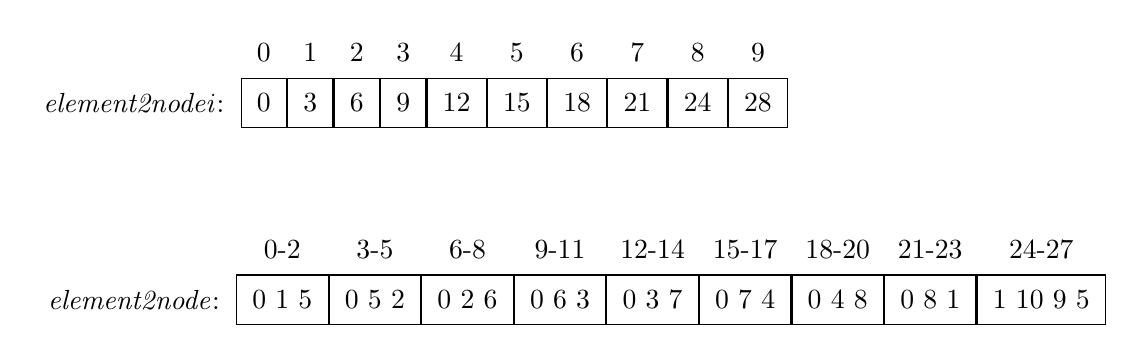
\begin{tikzpicture}[inner sep=2mm,minimum size = 2mm]
%Name
\node at(0,0) (namei) {\textit{element2nodei}:} ;
%Data 
\node at (namei.east)[rectangle,draw=black,right] (e0) {0} ;
\node at (e0.east)[rectangle,draw=black,right] (e1) {3} ;
\node at (e1.east)[rectangle,draw=black,right] (e2) {6} ;
\node at (e2.east)[rectangle,draw=black,right] (e3) {9} ;
\node at (e3.east)[rectangle,draw=black,right] (e4) {12} ;
\node at (e4.east)[rectangle,draw=black,right] (e5) {15} ;
\node at (e5.east)[rectangle,draw=black,right] (e6) {18} ;
\node at (e6.east)[rectangle,draw=black,right] (e7) {21} ;
\node at (e7.east)[rectangle,draw=black,right] (e8) {24} ;
\node at (e8.east)[rectangle,draw=black,right] (e9) {28} ;
%Address 
\node at (e0.north)[black,above] (a0) {0} ;
\node at (e1.north)[black,above] (a1) {1} ;
\node at (e2.north)[black,above] (a2) {2} ;
\node at (e3.north)[black,above] (a3) {3} ;
\node at (e4.north)[black,above] (a4) {4} ;
\node at (e5.north)[black,above] (a5) {5} ;
\node at (e6.north)[black,above] (a6) {6} ;
\node at (e7.north)[black,above] (a7) {7} ;
\node at (e8.north)[black,above] (a8) {8} ;
\node at (e9.north)[black,above] (a9) {9} ;

%Name
\node at (0,-2.5) (name) {\textit{element2node}:} ;
%Data 
\node at (name.east)[rectangle,draw=black,right] (d0) {0 1 5} ;
\node at (d0.east)[rectangle,draw=black,right] (d1) { 0 5 2 } ;
\node at (d1.east)[rectangle,draw=black,right] (d2) { 0 2 6 } ;
\node at (d2.east)[rectangle,draw=black,right] (d3) { 0 6 3 } ;
\node at (d3.east)[rectangle,draw=black,right] (d4) { 0 3 7 } ;
\node at (d4.east)[rectangle,draw=black,right] (d5) { 0 7 4 } ;
\node at (d5.east)[rectangle,draw=black,right] (d6) { 0 4 8 } ;
\node at (d6.east)[rectangle,draw=black,right] (d7) { 0 8 1 } ;
\node at (d7.east)[rectangle,draw=black,right] (d8) { 1 10 9 5 } ;
%Address 
\node at (d0.north)[black,above] (da0) {0-2} ;
\node at (d1.north)[black,above] (da1) {3-5} ;
\node at (d2.north)[black,above] (da2) {6-8} ;
\node at (d3.north)[black,above] (da3) {9-11} ;
\node at (d4.north)[black,above] (da4) {12-14} ;
\node at (d5.north)[black,above] (da5) {15-17} ;
\node at (d6.north)[black,above] (da6) {18-20} ;
\node at (d7.north)[black,above] (da7) {21-23} ;
\node at (d8.north)[black,above] (da8) {24-27} ;
%\draw [->] (e0.south) -- (da0.north);
%\draw [->] (e1.south) -- (da0.north);
\end{tikzpicture} 
\end{figure}

\bibliographystyle{unsrt}
\addcontentsline{toc}{chapter}{\bibname} % make reference section show up in TOC

% reads in the sample BibTex file supplied; change to your bib file name
\bibliography{fem}
\end{document}
